\def\DoNotLoadEpstopdf{}
\documentclass[tikz,border=4pt]{standalone}
% Shared style for the technical appendix figures (2026-10-26).
% Builds on the proposal's figstyle.tex (same fonts, colors, and box styles) and adds
% one encoding for development status, used the same way in every appendix figure.
%   built and tested   solid border (the proposal's normal box styles)
%   built, no test     solid border, and the box text says "no test"
%   specified          dashed border            -> add the key  spec
%   planned            dotted grey border        -> use the style planned
%   no code (by hand)  dotted arrow              -> add the key  byhand
%   outside the artifact  solid grey border      -> use the style outside
% Shared style for proposal figures (2026-10-22 visuals pass).
% Sized to print at 6.5 in (16.5 cm) wide; body text 9 pt sans, nothing below 8 pt.
\usepackage[T1]{fontenc}
\usepackage[scaled=0.95]{helvet}
\renewcommand{\familydefault}{\sfdefault}
\usepackage{xcolor}
\usetikzlibrary{arrows.meta,positioning,calc,patterns.meta}
\definecolor{cink}{HTML}{16191F}
\definecolor{cmuted}{HTML}{4B5563}
\definecolor{cslate}{HTML}{2F4858}
\definecolor{cslatefill}{HTML}{E9EFF3}
\definecolor{cbrass}{HTML}{7A5C12}
\definecolor{cbrassfill}{HTML}{F5EFDE}
\definecolor{cred}{HTML}{8C2F39}
\definecolor{credfill}{HTML}{F8E9EA}
\definecolor{cgreen}{HTML}{235C53}
\definecolor{cgreenfill}{HTML}{E3F0EC}
\definecolor{caudit}{HTML}{5B3A8E}
\definecolor{cauditfill}{HTML}{EFE9F6}
\definecolor{cghost}{HTML}{6B7280}
\definecolor{cghostfill}{HTML}{F3F4F6}
\tikzset{
  >={Triangle[length=5pt,width=4.5pt]},
  box/.style={draw, rounded corners=1.5pt, line width=0.8pt, align=center, inner sep=4pt, font=\fontsize{9}{11}\selectfont},
  sub/.style={font=\fontsize{8}{9.6}\selectfont, text=cmuted},
  ai/.style={box, draw=cbrass, fill=cbrassfill, text=cbrass},
  ver/.style={box, draw=cred, fill=credfill, text=cred},
  pipe/.style={box, draw=cslate, fill=cslatefill, text=cslate},
  prod/.style={box, draw=cslate, fill=cslate, text=white},
  person/.style={box, draw=cink, fill=white, text=cink},
  ghost/.style={box, draw=cghost, fill=cghostfill, text=cghost, dash pattern=on 3pt off 2pt},
  flow/.style={->, line width=0.8pt},
}

\renewcommand{\ttdefault}{lmtt}% vector typewriter font (same design as the default, not a bitmap)
\tikzset{
  spec/.style={dash pattern=on 3pt off 2pt},
  planned/.style={box, draw=cghost, fill=cghostfill, text=cghost, dash pattern=on 0.9pt off 1.6pt},
  outside/.style={box, draw=cghost, fill=white, text=cghost},
  byhand/.style={dash pattern=on 0.9pt off 1.6pt},
  prog/.style={font=\fontsize{8}{9.6}\selectfont\ttfamily},
  legendbox/.style={draw, rounded corners=1pt, line width=0.8pt, minimum width=0.55cm, minimum height=0.32cm, inner sep=0pt},
  legendtext/.style={font=\fontsize{8}{9.6}\selectfont, text=cink, anchor=west, inner sep=1pt},
}
% \statuslegend{x}{y} draws the four-item status legend with its left edge at (x,y).
\newcommand{\statuslegend}[2]{%
  \begin{scope}[shift={(#1,#2)}]
    \node[legendbox, draw=cink, fill=white] (lg1) at (0.275,0) {};
    \node[legendtext] at (0.65,0) {Built and tested};
    \node[legendbox, draw=cink, fill=white, spec] (lg2) at (3.35,0) {};
    \node[legendtext] at (3.725,0) {Specified};
    \node[legendbox, draw=cghost, fill=cghostfill, dash pattern=on 0.9pt off 1.6pt] (lg3) at (5.75,0) {};
    \node[legendtext] at (6.125,0) {Planned};
    \node[legendbox, draw=cghost, fill=white] (lg4) at (7.85,0) {};
    \node[legendtext] at (8.225,0) {Outside the research artifact};
  \end{scope}}

% The README's figure: the proposal's layer figure filled in with what the workflow
% found about the proposal and its appendix. Counts are from the reports in verification/.
\begin{document}
\hyphenpenalty=10000
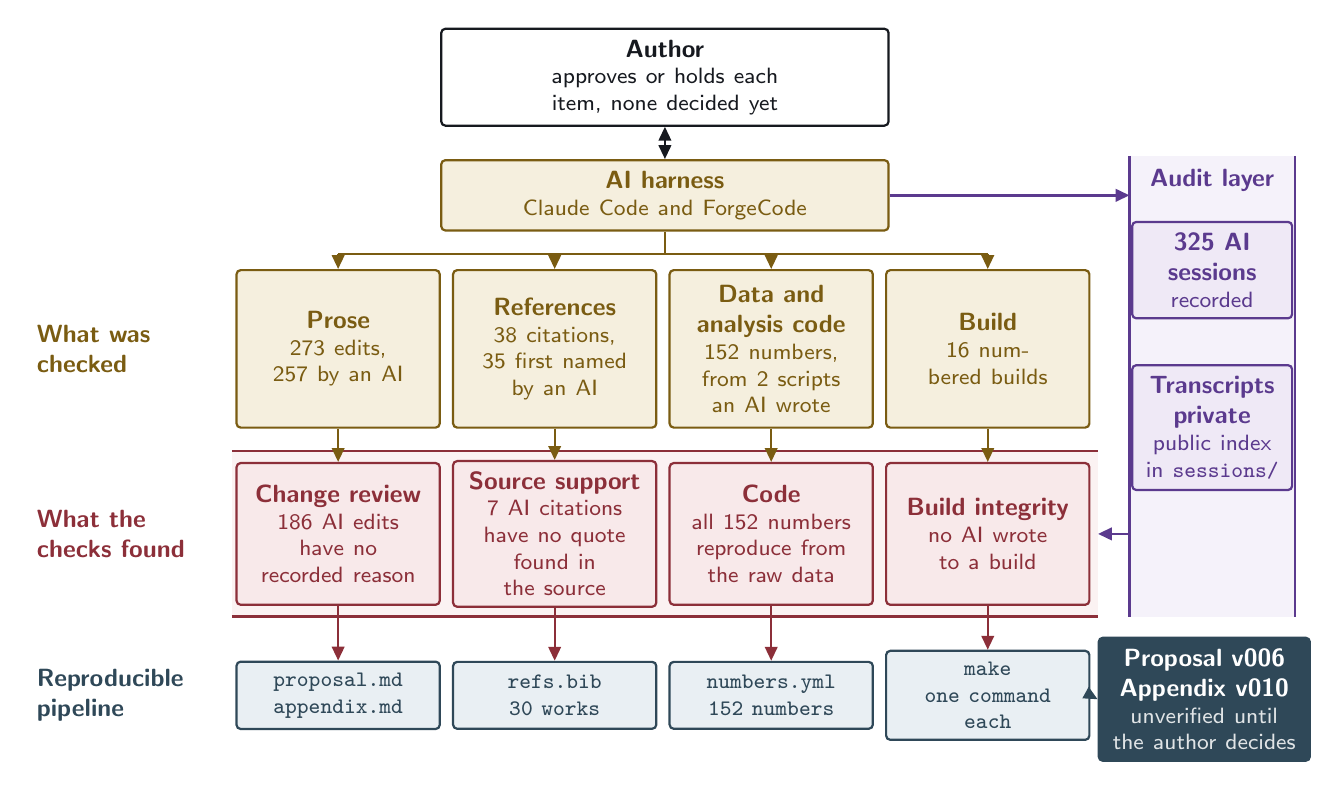
\begin{tikzpicture}
\tikzset{lab/.style={font=\fontsize{9}{11}\selectfont\bfseries, anchor=west, align=left, text width=2.4cm},
         col/.style={minimum width=2.5cm, text width=2.3cm, font=\fontsize{9}{11}\selectfont\bfseries}}
\newcommand{\pg}[1]{{\fontsize{8}{9.6}\selectfont\ttfamily\mdseries #1\par}}
\newcommand{\sm}[1]{{\fontsize{8}{9.6}\selectfont\mdseries #1\par}}
\foreach \i in {0,1,2,3} {\pgfmathsetmacro{\x}{3.95+2.75*\i}\expandafter\xdef\csname cx\i\endcsname{\x}}
% author
\node[person, col, minimum width=5.6cm, text width=5.4cm, minimum height=0.8cm] (sch) at (8.1,2.9) {Author\par\sm{approves or holds each item, none decided yet}};
% AI harness
\node[ai, col, minimum width=5.6cm, text width=5.4cm, minimum height=0.8cm] (h) at (8.1,1.4) {AI harness\par\sm{Claude Code and ForgeCode}};
\draw[<->, line width=0.8pt, cink] (sch.south) -- (h.north);
% audit band
\fill[cauditfill!60!white] (14.0,1.9) rectangle (16.1,-3.95);
\draw[caudit, line width=0.8pt] (14.0,1.9) -- (14.0,-3.95) (16.1,1.9) -- (16.1,-3.95);
\node[font=\fontsize{9}{11}\selectfont\bfseries, text=caudit, anchor=north, align=center] at (15.05,1.85) {Audit layer};
\tikzset{aui/.style={box, draw=caudit, fill=cauditfill, text=caudit, minimum width=1.9cm, text width=1.75cm, minimum height=0.75cm, font=\fontsize{9}{11}\selectfont\bfseries}}
\node[aui] at (15.05,0.45) {325 AI sessions\par\sm{recorded}};
\node[aui] at (15.05,-1.55) {Transcripts private\par\sm{public index in \texttt{sessions/}}};
\draw[->, line width=0.9pt, caudit] (h.east) -- (14.0,0 |- h.east);
\draw[->, line width=0.9pt, caudit] (14.0,-2.9) -- (13.6,-2.9);
% what was checked
\draw[line width=0.8pt, cbrass] (h.south) -- (8.1,0.65);
\draw[line width=0.8pt, cbrass] (3.95,0.65) -- (12.2,0.65);
\node[lab, text=cbrass] at (0,-0.55) {What was checked};
\foreach \i/\t/\u in {0/Prose/{273 edits, 257 by an AI}, 1/References/{38 citations, 35 first named by an AI}, 2/Data and analysis code/{152 numbers, from 2 scripts an AI wrote}, 3/Build/{16 numbered builds}} {
  \node[ai, col, minimum height=2.0cm] (s\i) at (\csname cx\i\endcsname,-0.55) {\t\par\sm{\u}};
  \draw[flow, cbrass] (\csname cx\i\endcsname,0.65) -- (s\i.north);
}
% verification layer
\fill[credfill!60!white] (2.6,-1.85) rectangle (13.6,-3.95);
\draw[cred, line width=0.8pt] (2.6,-1.85) -- (13.6,-1.85) (2.6,-3.95) -- (13.6,-3.95);
\node[lab, text=cred] at (0,-2.9) {What the checks found};
\foreach \i/\t/\u in {0/Change review/{186 AI edits have no recorded reason}, 1/Source support/{7 AI citations have no quote found in the source}, 2/Code/{all 152 numbers reproduce from the raw data}, 3/Build integrity/{no AI wrote to a build}} {
  \node[ver, col, minimum height=1.8cm] (v\i) at (\csname cx\i\endcsname,-2.9) {\t\par\sm{\u}};
  \draw[flow, cbrass] (s\i.south) -- (v\i.north);
}
% reproducible pipeline
\node[lab, text=cslate] at (0,-4.95) {Reproducible pipeline};
\foreach \i/\t/\u in {0/proposal.md/appendix.md, 1/refs.bib/30 works, 2/numbers.yml/152 numbers, 3/make/one command each} {
  \node[pipe, col, font=\fontsize{9}{11}\selectfont, minimum height=0.85cm] (p\i) at (\csname cx\i\endcsname,-4.95) {\pg{\t}\pg{\u}};
  \draw[flow, cred] (v\i.south) -- (p\i.north);
}
\node[prod, col, minimum width=2.6cm, text width=2.4cm, minimum height=1.0cm] (rp) at (14.95,-5.0) {Proposal v006\par Appendix v010\par{\fontsize{8}{9.6}\selectfont\mdseries\color{white!85!cslate} unverified until the author decides\par}};
\draw[flow, cslate] (p3.east) -- (rp.west);
\end{tikzpicture}
\end{document}
